    %\ifx\isEmbedded\undefined
%	% Loading common settings
%	\input{macros/common}
%	% Loading common variable definitions 
%	\input{macros/macros}
%	\begin{document} 
%\else
%\fi
%



%\setcounter{chapter}{1}

\chapter{A Simple Vision System}
\label{chapter:simplesystem}

\section{Introduction}

The goal of this chapter is to embrace the optimism of the 1960s and to hand-design an end-to-end visual system. During this process, we will cover some of the main concepts that will be developed in the rest of the book. 


In 1966, Seymour Papert wrote a proposal for building a vision system as a summer project \cite{Papert66}. The abstract of the proposal starts by stating a simple goal: ``The summer vision project is an attempt to use our summer workers effectively in the construction of a significant part of a visual system.'' The report then continues dividing all the tasks (most of which also are common parts of modern computer vision approaches) among a group of MIT students. This project was a reflection of the optimism existing in the early days of computer vision. However, the task proved to be harder than anybody expected.  

In this first chapter, we will discuss several of the main topics that we will cover in this book. We will do this in the framework of a real, although a bit artificial, vision problem. Vision has many different goals (e.g., object recognition, scene interpretation, three-dimensional [3D] interpretation), but in this chapter we're just focusing on the task of 3D interpretation.

\section{A Simple World: The Blocks World}


As the visual world is too complex, we will start by simplifying it enough that we will be able to build a simple visual system right away. This was the strategy used by some of the first scene interpretation systems.  Larry G. Roberts \cite{Roberts63} introduced the {\bf Block world}, a world composed of simple 3D geometrical figures. 
\index{Block world}
\marginnote{Blocks world from Larry Roberts' Ph.D. in June 1963.
\\[6pt]
\centerline{
\setlength{\fboxsep}{0pt}
\fbox{\includegraphics[width=.4\linewidth]{figures/simplesystem/roberts_phd_figure.eps}}
} 
}

For the purposes of this chapter, let's think of a world composed of a very simple (yet varied) set of objects. These simple objects are composed of flat surfaces that can be horizontal or vertical. These objects will be resting on a white horizontal ground plane. We can build these objects by cutting, folding, and gluing together some pieces of colored paper as shown in \fig{\ref{fig:simpleObjects}}. Here, we will not assume that we know the exact geometry of these objects in advance. 

\begin{figure}[t]
\centerline{
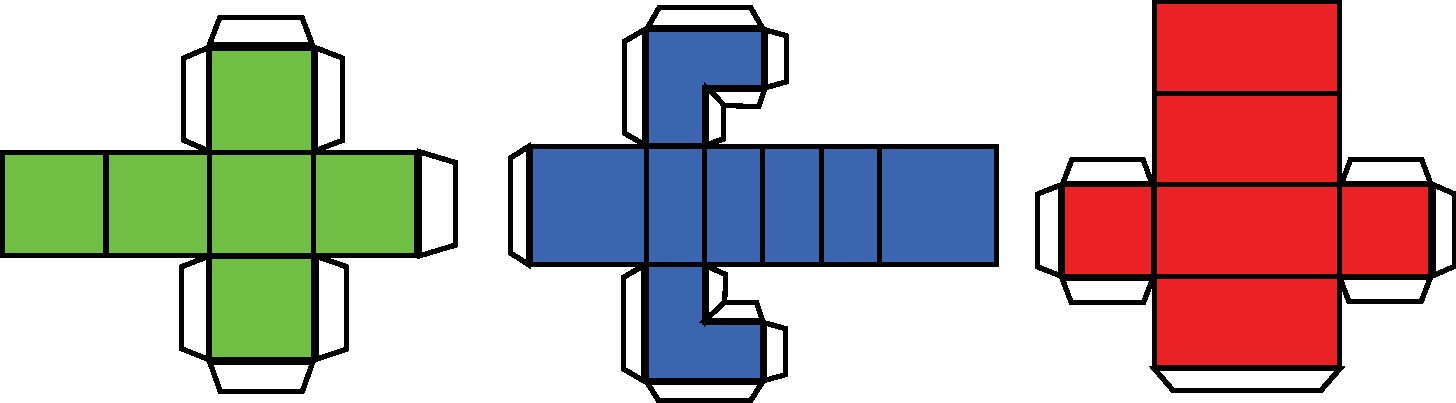
\includegraphics[width=1\linewidth]{figures/simplesystem/simpleObjects.pdf}
} 
\caption{A world of simple objects. Print, cut, and build your own blocks world!} 
\label{fig:simpleObjects}
\end{figure}



\section{A Simple Image Formation Model}

One of the simplest forms of projection is {\bf parallel} (or {\bf orthographic}) {\bf projection}\index{Parallel projection}. In this image formation model, the light rays travel parallel to each other and perpendicular to the camera plane. This type of projection produces images in which objects do not change size as they move closer or farther from the camera, and parallel lines in 3D remain  parallel in the 2D image.  This is different from the perspective projection, to be discussed in \sect{\ref{sec:pinhole_camera_formation}}, where the image is formed by the convergence of the light rays into a single point (focal point). If we do not take special care, most pictures taken with a camera will be better described by {\bf perspective projection}\index{Perspective projection}, as shown in \fig{\ref{fig:parallelProjection}}{a}.  


\begin{figure}[t]
\centerline{
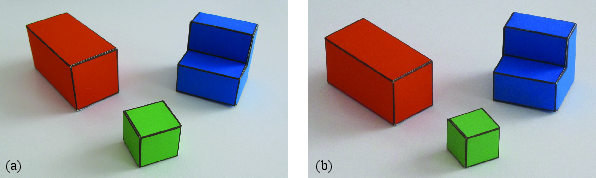
\includegraphics[width=1\linewidth]{figures/simplesystem/parallelProjection.pdf}
} 
\caption{(a) Close up picture without zoom. Note that near edges are larger than far edges, and parallel lines in 3D are not parallel. (b) Picture taken from far away using zoom resulting in an image that can be described by parallel projection.} 
\label{fig:parallelProjection}
\end{figure}

One way of generating images that can be described by parallel projection is to use the camera zoom. If we increase the distance between the camera and the object while zooming, we can keep the same approximate image size of the objects, but with reduced perspective effects, as shown in \fig{\ref{fig:parallelProjection}}{b}. Note how, in \fig{\ref{fig:parallelProjection}}{b}, 3D parallel lines in the world are almost parallel in the image (some weak perspective effects remain). 
\marginnote{Changing the zoom to compensate a moving camera can be used to create movie effects. This method was introduced by Alfred Hitchcock to create a sequence, centered in a subject, where the background moves away or closer to the subject.}[-.1in]


The first step is to characterize how a point in world coordinates $(X,Y,Z)$ projects into the image plane. \Fig{\ref{fig:projection}}{a} shows our parameterization of the world and the camera coordinate systems. The camera center is inside the 3D plane $X=0$, and the horizontal axis of the camera ($x$) is parallel to the ground plane ($Y=0$). The camera is tilted so that the line connecting the origin of the world coordinates system and the image center is perpendicular to the image plane. The angle $\theta$ is the angle between this line and the $Z$-axis. The image is parameterized by coordinates $(x,y)$. 

\begin{figure}[t]
\centerline{
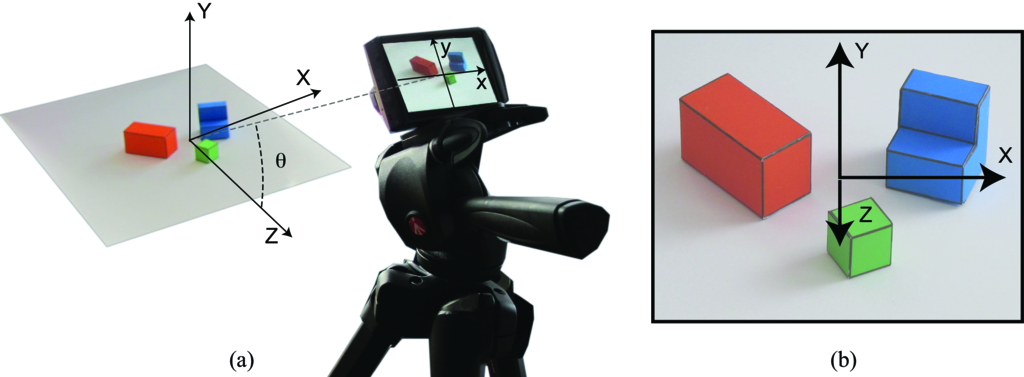
\includegraphics[width=1\linewidth]{figures/simplesystem/projection2.eps}
} 
\caption{A simple projection model. (a) World axis and camera plane. (b) Visualization of the world axis projected into the camera plane with parallel projection. The $Z$-axis is identical to the $Y$-axis up to a sign change and a scaling.} 
\label{fig:projection}
\end{figure}

In this simple projection model, the origin of the world coordinates projects on the origin of the image coordinates. Therefore, the world point $(0,0,0)$ projects into $(0,0)$.
%The center of the image is at coordinates $(x_0, y_0)$. 
The resolution of the image (the number of pixels) will also affect the transformation from world coordinates to image coordinates via a constant factor $\alpha$ (for now we assume that pixels are square and we will see a more general form in \sect{\ref{sec:camera_parameters}}) and that this constant is $\alpha=1$. Taking into account all these assumptions, the transformation between world coordinates and image coordinates can be written as follows: 
\begin{eqnarray}
x &=& X \\
y &=&  \cos(\theta) Y - \sin(\theta) Z 
% &=& \alpha X + x_0\\
%y &=& \alpha( \cos(\theta) Y - \sin(\theta) Z ) + y_0
\label{eq:projection}
\end{eqnarray}




With this particular parametrization of the world and camera coordinate systems, the world coordinates $Y$ and $Z$ are mixed after projection.  From the camera, a point moving parallel to the $Z$-axis will be indistinguishable from a point moving parallel to the $Y$-axis.


\section{A Simple Goal}

Part of the simplification of the vision problem resides in simplifying its goals. In this chapter we will focus on recovering the world coordinates of all the pixels seen by the camera. 

Besides recovering the 3D structure of the scene, there are many other possible goals that we will not consider in this chapter. For instance, one goal (which might seem simpler but is not) is to recover the actual color of the surface seen by each pixel $(x,y)$. This will require discounting for illumination effects as the color of the pixel is a combination of the surface albedo and illumination (color of the light sources and interreflections). 


\section{From Images to Edges and Useful Features}
\label{sec:algo_simple_world}


The observed image is a function, 
\begin{equation}
\img(x,y) 
\end{equation}
that takes as input location, $(x,y)$, and it outputs the intensity at that location. In this {\bf representation}, the image is an array of intensity values (color values) indexed by location (\fig{\ref{fig:imageAsSurface}}). 


\begin{figure}[t]
\centerline{
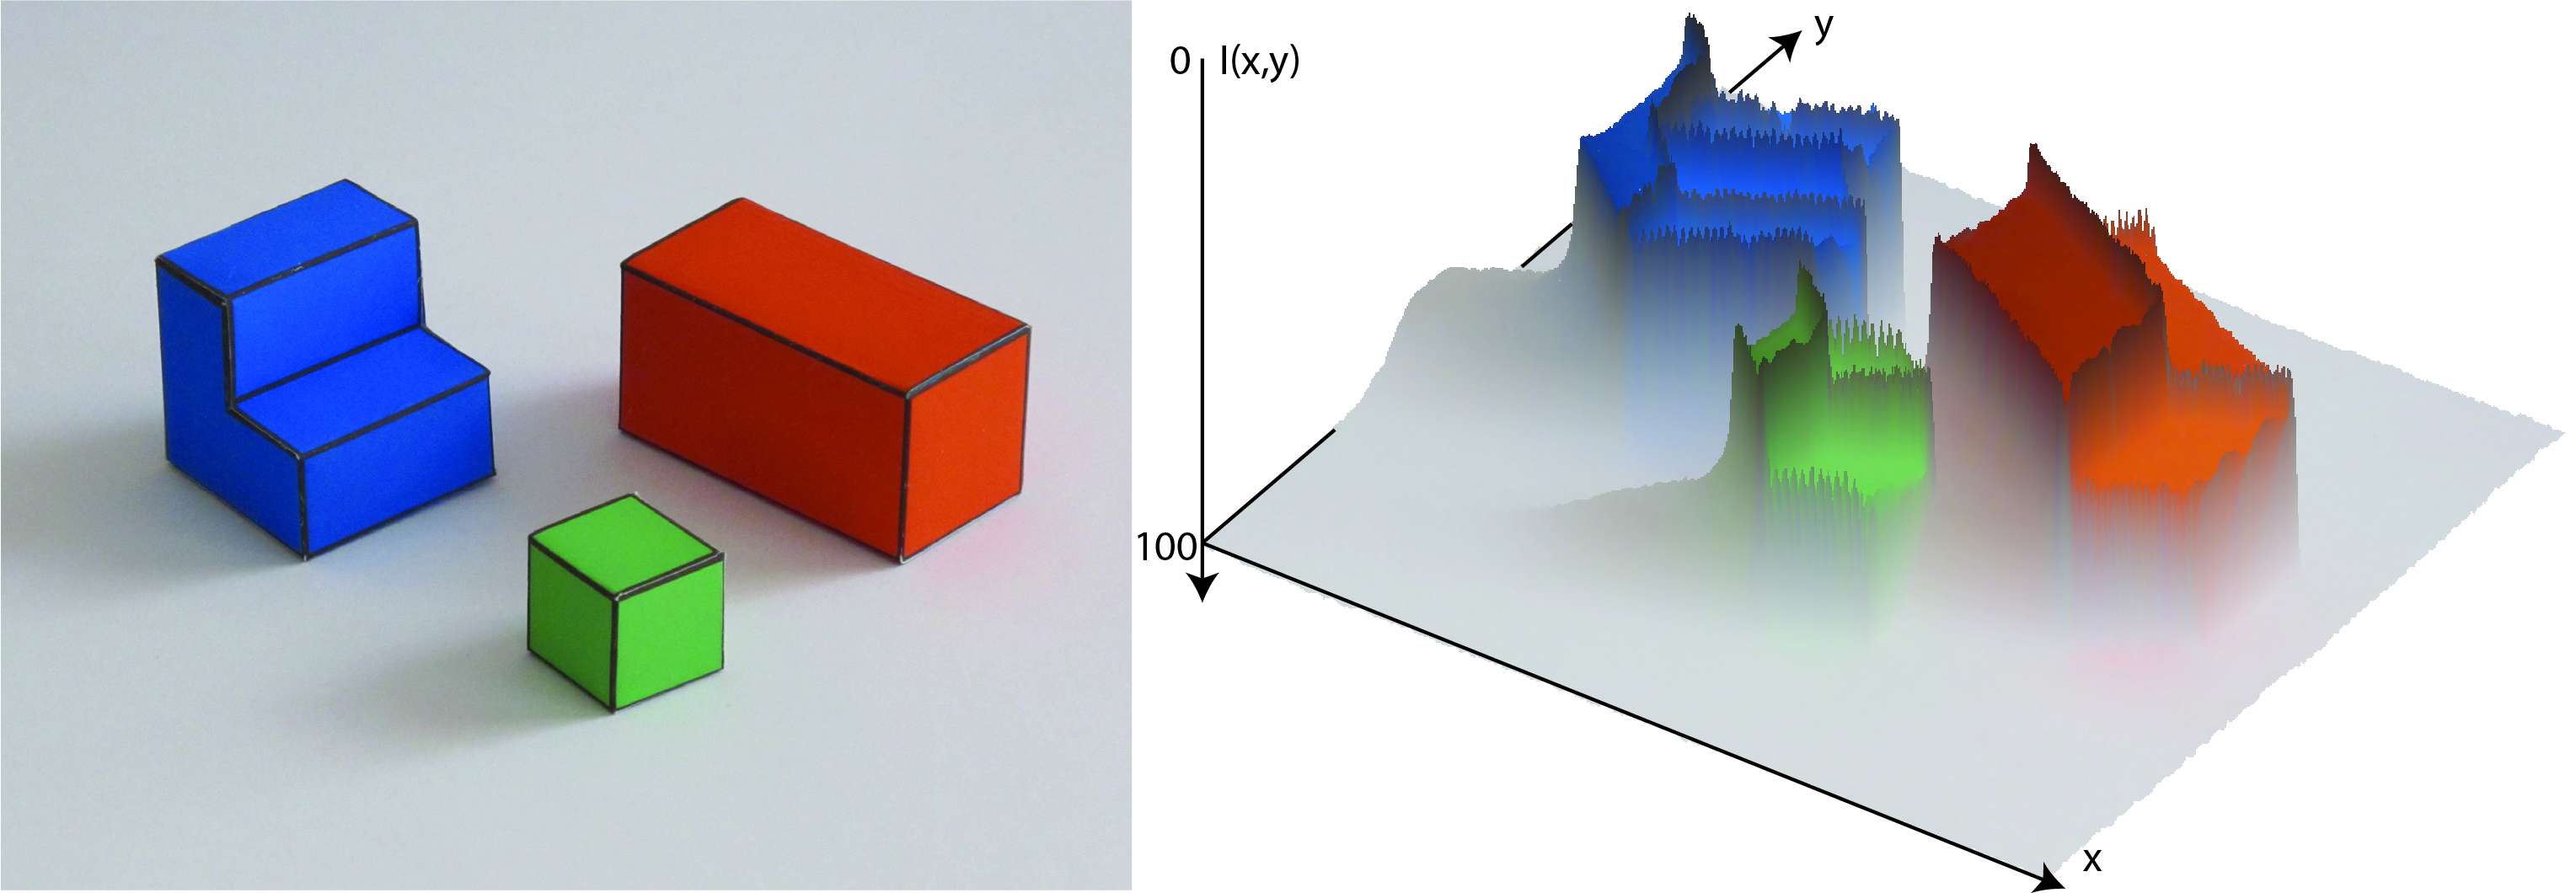
\includegraphics[width=1\linewidth]{figures/simplesystem/imageAsSurface.jpg}
} 
\caption{Image as a surface. The vertical axis corresponds to image intensity. For clarity here, we have reversed the vertical axis. Dark values are shown higher than lighter values.} 
\label{fig:imageAsSurface}
\end{figure}

%This representation is great if we are interested in knowing the light intensity coming from each direction of the space and striking the camera plane, as this information is explicitly represented. 
This representation is ideal for determining the light intensity originating from different directions in space and striking the camera plane, as it provides explicit representation of this information. The array of pixel intensities, $\img(x,y)$, is a reasonable representation as input to the early stages of visual processing because, although we do not know the distance of surfaces in the world, the direction of each light ray in the world is well defined. However, other initial representations could be used by the visual system (e.g., images could be coded in the Fourier domain, or pixels could combine light coming in different directions). 


However, in the simple visual system of this chapter we are interested in interpreting the 3D structure of the scene and the objects within. Therefore, it will be useful to transform the image into a representation that makes more explicit some of the important parts of the image that carry information about the boundaries between objects and changes in the surface orientation. 

%The representation will not be unique. Different levels of the scene understanding process will rely on different representations. 





% 
%Murphy, C. J., & Howland, H. C. (1986). On the gekko pupil and Scheiner's disc. Vision Research, 26(5), 815–817. https://doi.org/10.1016/0042-6989(86)90097-0
%
% https://asknature.org/strategy/pupil-enables-clear-vision-in-extreme-light-conditions/
There are several representations that can be used as an initial step for scene interpretation. Images can be represented as collections of small image patches, regions of uniform properties, and edges. 


\marginnote{{\bf Question}: Are there animal eyes that produce a different initial representations than ours? 
{\bf Answer}: Yes! One example is the Gekko's eye. Their pupil has a four-diamond-shaped pinhole aperture that could allow them to encode distance to a target in the retinal image \cite{Murphy1986}. Photo credit: \cite{Randall}. \\[6pt]
\centerline{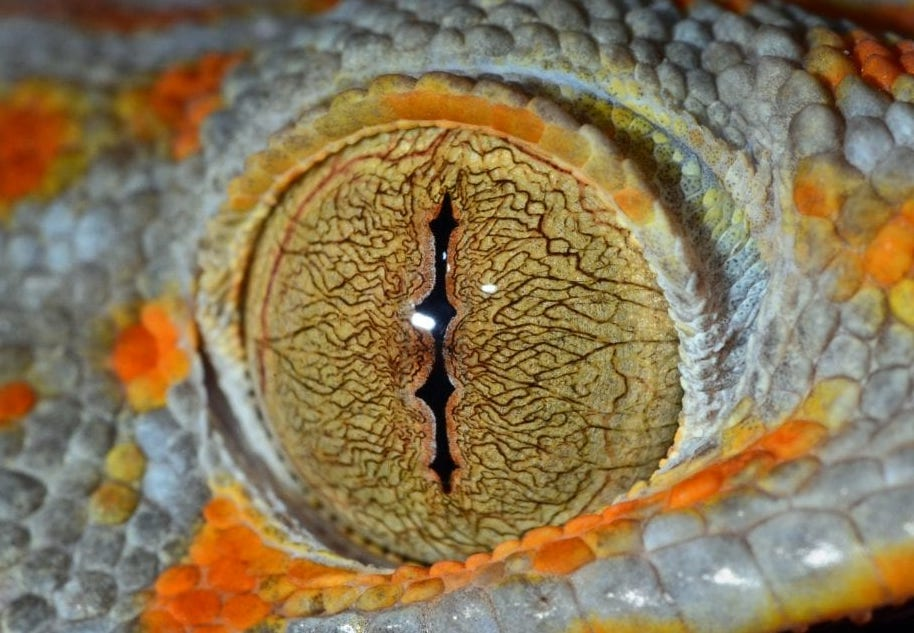
\includegraphics[width=.4\linewidth]{figures/simplesystem/Tokay-Gecko-Eye-1440x954.jpg}} 
}[-4cm]

\subsection{A Catalog of Edges}

Edges denote image regions where there are strong changes of the image  with respect to location. Those variations can be due to a multitude of scene factors (e.g., occlusion boundaries, changes in surface orientation, changes in surface albedo, shadows).

\begin{figure}[t]
\centerline{
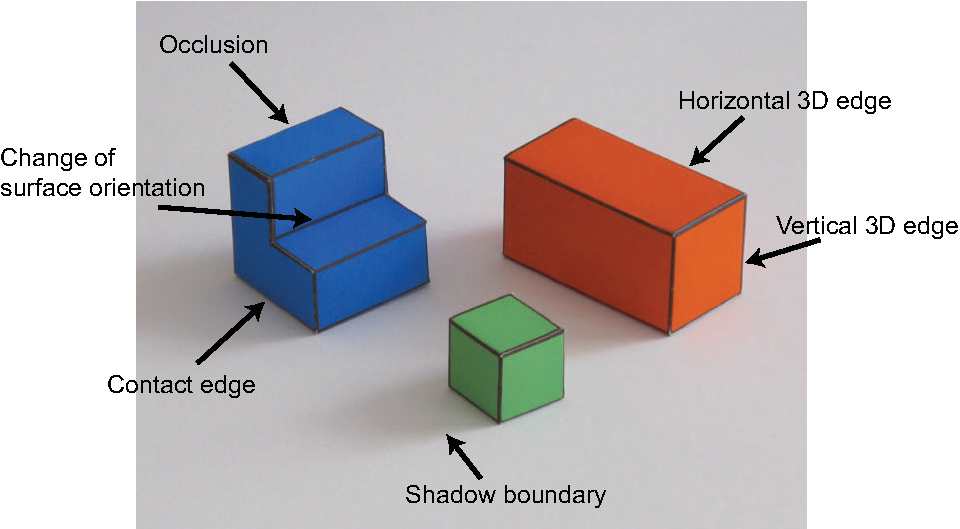
\includegraphics[width=.9\linewidth]{figures/simplesystem/edgeLabeling.pdf}
} 
\caption{Edges denote image regions where there are sharp changes of the image intensities. Those variations can be due to a multitude of scene factors (e.g., occlusion boundaries, changes in surface orientation, changes in surface albedo, and shadows).} 
\label{fig:edgeLabeling}
\end{figure}

One of the tasks that we will solve first is to classify {\bf image edges}\index{Edge!types} according to their most probable cause. We will use the following classification of image boundaries (\fig{\ref{fig:edgeLabeling}}):
\begin{itemize}
\item {\bf Object boundaries}: These indicate pixels that delineate the boundaries of any object. Boundaries between objects generally correspond to changes in surface color, texture, and orientation. 

\item Changes in {\bf surface orientation}: These indicate locations where there are strong image variations due to changes in the surface orientations. A change in surface orientation produces changes in the image intensity because intensity is a function of the angle between the surface and the incident light.  

\item {\bf Shadow edges}: This can be harder than it seems. In this simple world, shadows are soft, creating slow transitions between dark and light.
\end{itemize}

We will also consider two types of object boundaries:
\begin{itemize}
\item {\bf Contact edges}: This is a boundary between two objects that are in physical contact. Therefore, there is no depth discontinuity. 

\item {\bf Occlusion boundaries}: Occlusion boundaries happen when an object is partially in front of another. Occlusion boundaries generally produce depth discontinuities. In this simple world, we will position the objects in such a way that objects do not occlude each other but they will occlude the background.
\end{itemize}

Despite the apparent simplicity of this task, in most natural scenes, this classification is very hard and requires the interpretation of the scene at different levels. In other chapters we will see how to make better edge classifiers (i.e., by propagating information along boundaries, junction analysis, inferring light sources).


\subsection{Extracting Edges from Images}

The first step will consist in detecting candidate edges in the image.
\index{Edge!detection}
%We will describe other techniques in detail in lecture 14. 
Here we will start by making use of some notions from differential geometry. If we think of the image $\img (x,y)$ as a function of two (continuous) variables (\fig{\ref{fig:imageAsSurface}}), we can measure the degree of variation using the gradient:
\begin{eqnarray}
\nabla \img = \left( \frac{\partial \img}{\partial x}, \frac{\partial \img}{\partial y} \right)
\end{eqnarray}
The direction of the gradient indicates the direction in which the variation of intensities is larger. If we are on top of an edge, the direction of larger variation will be in the direction perpendicular to the edge. 

\marginnote{Gradient of an image at one location:
\\~\\
\centerline{\includegraphics[width=.35\linewidth]{figures/simplesystem/gradient2.eps}
} 
}[-0.5in]

However, the image is not a continuous function as we only know the values of the $\img (x,y)$ at discrete locations (pixels). Therefore, we will approximate the partial derivatives by:
\begin{eqnarray}
\frac{\partial \img}{\partial x} & \simeq & \img(x,y) - \img(x-1,y) \\
\frac{\partial \img}{\partial y} & \simeq & \img(x,y) - \img(x,y-1) 
\label{eq:image_partial_derivatives_aprox}
\end{eqnarray}

A better behaved approximation of the partial image derivative can be computed by combining the image pixels around $(x,y)$ with the weights:
\begin{eqnarray}
\frac{1}{4} \times
\left [
\begin{matrix}
-1 & 0 & 1 \\
-2 & 0 & 2 \\
-1 & 0 & 1 
\end{matrix}
\right ] \nonumber
\end{eqnarray}
We will discuss these approximations in detail in \chap{\ref{chapter:image_derivatives}}. 

From the image gradient, we can extract a number of interesting quantities:
\index{Edge!strength} \index{Edge!orientation}
\begin{align}
    e(x,y) &= \lVert \nabla \img(x,y) \rVert   & \quad\quad \triangleleft \quad \texttt{edge strength}\\
    \theta(x,y) &= \angle \nabla \img =  \arctan \left( \frac{\partial \img / \partial y}{\partial \img / \partial x} \right) & \quad\quad \triangleleft \quad \texttt{edge orientation}
\end{align}
\marginnote{The edge strength is the gradient magnitude, and the edge orientation is perpendicular to the gradient direction.}

The unit norm vector perpendicular to an edge is:
\begin{eqnarray}
{\bf n} = \frac{\nabla \img}{\lVert \nabla \img \rVert}
\end{eqnarray}



%\subsection{Edge classification}



The first decision that we will perform is to decide which pixels correspond to edges (regions of the image with sharp intensity variations) and which ones belong to uniform regions (flat surfaces). We will do this by simply thresholding the edge strength $e(x,y)$. 
%In lecture 14 we will discuss more sophisticated edge detectors. 
In the pixels with edges, we can also measure the edge orientation $\theta(x,y)$. \Fig{\ref{fig:gradient}} visualizes the edges and the normal vector on each edge. 


\begin{figure}[t]
\centerline{
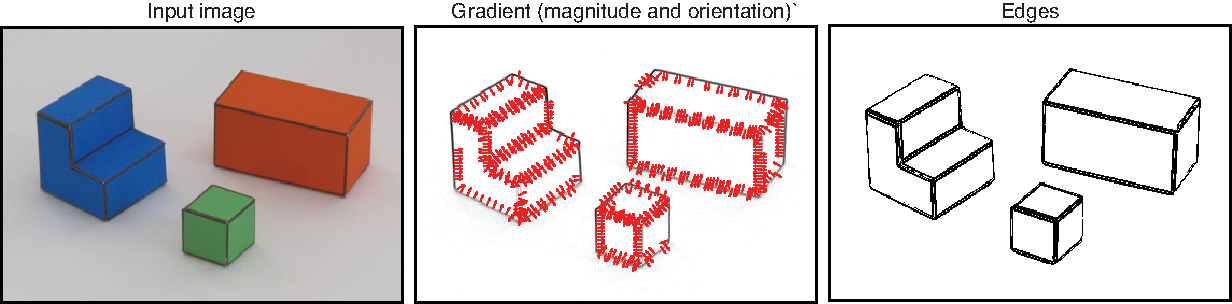
\includegraphics[width=1\linewidth]{figures/simplesystem/gradient.pdf}
} 
\centerline{
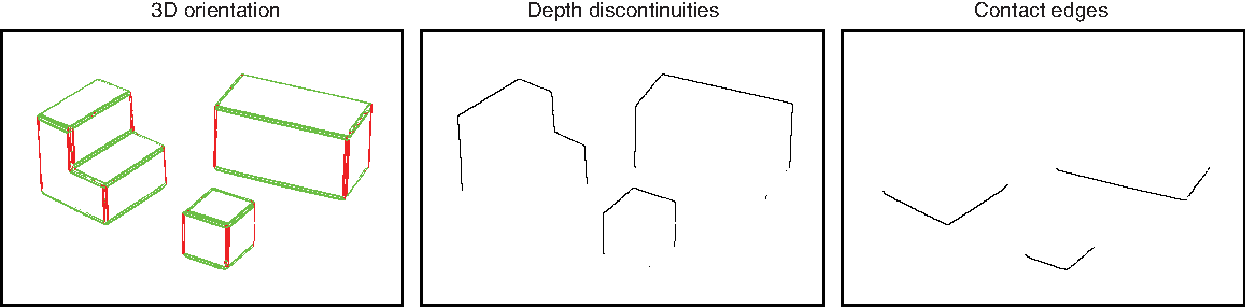
\includegraphics[width=1\linewidth]{figures/simplesystem/edgeTypes.pdf}
} 
\caption{Gradient and edge types.} 
\label{fig:gradient}
\end{figure}

\section{From Edges to Surfaces}

We want to recover world coordinates $X(x,y)$, $Y(x,y)$, and $Z(x,y)$ for each image location $(x,y)$. Given the simple image formation model described before, recovering the $X$ world coordinates is trivial as they are directly observed: for each pixel with image coordinates $(x,y)$, the corresponding world coordinate is $X(x,y) = x$. Recovering $Y$ and $Z$ will be harder as we only observe a mixture of the two world coordinates (one dimension is lost due to the projection from the 3D world into the image plane). Here we have written the world coordinates as functions of image location $(x,y)$ to make explicit that we want to recover the 3D locations of the visible points. 

In this simple world, we will formulate this problem as a set of linear equations. 



\subsection{Figure/Ground Segmentation}



Segmentation of an image into figure and ground is a classical problem in human perception and computer vision that was introduced by {\bf Gestalt psychology}.\index{Gestalt psychology}

\marginnote{The classical visual illusion ``two faces or a vase'' is an example of {\bf figure-ground} segmentation problem.\\[6pt]
\centerline{

\includegraphics[width=.4\linewidth]{figures/simplesystem/figure-ground.eps}
}}

In this simple world deciding when a pixel belongs to one of the {\bf foreground} objects or to the {\bf background} can be decided by simply looking at the color values of each pixel. Bright pixels that have low saturation (similar values of the red-blue-green [RBG] components) correspond to the white ground plane, and the rest of the pixels are likely to belong to the colored blocks that compose our simple world. In general, the problem of {\bf image segmentation} into distinct objects is a very challenging task.% that we will study in lecture 9. 

Once we have classified pixels as ground or figure, if we assume that the background corresponds to a horizontal ground plane, then for all pixels that belong to the ground we can set $Y(x,y)=0$. For pixels that belong to objects we will have to measure additional image properties before we can deduce any geometric scene constraints. 



\subsection{Occlusion Edges}

An occlusion boundary separates two different surfaces at different distances from the observer. 
Along an occlusion edge, it is also important to know which object is in front as this will be the one owning the boundary. Knowing who owns the boundary
 is important as an edge provides cues about the 3D geometry, but those cues only apply to the surface that owns the boundary. 
 \marginnote{{\bf Border ownership}: The foreground object is the one that owns the common edge.\\[6pt]
\centerline{
\includegraphics[width=.4\linewidth]{figures/simplesystem/border_ownership.eps}
}
The dotted lines belong to the object in front.
}

In this simple world, we will assume that objects do not occlude each other (this can be relaxed) and that the only occlusion boundaries are the boundaries between the objects and the ground. However, as we describe subsequently, not all boundaries between the objects and the ground correspond to depth gradients.



\subsection{Contact Edges}

Contact edges are boundaries between two distinct objects but where there exists no depth discontinuity. Despite that there is not a depth discontinuity, there is an occlusion here (as one surface is hidden behind another), and the edge shape is only owned by one of the two surfaces. 

In this simple world, if we assume that all the objects rest on the ground plane, then we can set $Y(x,y)=0$ on the contact edges.
Contact edges can be detected as transitions between the object (above) and ground (below). In our simple world only horizontal edges can be contact edges. We will discuss next how to classify edges according to their 3D orientation.


\begin{figure}
\centerline{
\includegraphics[width=.5\linewidth]{figures/simplesystem/ground_figure_points.eps}
} 
\caption{For each vertical line (shown in red), scanning from top to bottom, transitions from ground to figure are occlusion boundaries, and transitions from figure to ground are contact edges. This heuristic will fails when an object occludes another.} 
\label{fig:ground_figure_points}
\end{figure}

\subsection{Generic View and Nonaccidental Scene Properties}

Despite that in the projection of world coordinates to image coordinates we have lost a great deal of information, there are a number of properties that will remain invariant and can help us in interpreting the image. Here is a list of some of those invariant properties:
\begin{itemize}
\item Collinearity: a straight 3D line will project into a straight line in the image.
\item Cotermination: if two or more 3D lines terminate at the same point, the corresponding projections will also terminate at a common point. 
%\item Intersection: if two 3D lines intersect at a point, the projection will result in two intersecting lines.
%\item Parallelism: (under weak perspective)
%\item Symmetry: (under weak perspective)
\item Smoothness: a smooth 3D curve will project into a smooth 2D curve.
\end{itemize}
\marginnote{
\centerline{\includegraphics[width=.7\linewidth]{figures/simplesystem/invariants2.eps}} 
}
%% [FIGURE: show some 3D lines and 2D projections illustrating accidental alignments]

Note that those invariances refer to the process of going from world coordinates to image coordinates. The opposite might not be true. For instance, a straight line in the image could correspond to a curved line in the 3D world but that happens to be precisely aligned with respect to the viewers point of view to appear as a straight line. Also, two lines that intersect in the image plane could be disjointed in the 3D space. 


However, some of these properties (not all), while not always true, can nonetheless be used to reliably infer something about the 3D world using a single 2D image as input. For instance, if two lines coterminate in the image, then, one can conclude that it is very likely that they also touch each other in 3D. If the 3D lines do not touch each other, then it will require a very specific alignment between the observer and the lines  for them to appear to coterminate in the image. Therefore, one can safely conclude that the lines might also touch in 3D. 

These properties are called {\bf nonaccidental properties}\index{Nonaccidental image properties} \cite{Lowe1985} because they will only be observed in the image if they also exist in the world or by accidental alignments between the observer and scene structures. Under a {\bf generic view}\index{Generic view}, nonaccidental properties will be shared by the image and the 3D world \cite{Freeman94b}. 

Let's see how this idea applies to our simple world. In this simple world all 3D edges are either vertical or horizontal.  Under parallel projection and with the camera having its horizontal axis parallel to the ground, we know that vertical 3D lines will project into vertical 2D lines in the image. Conversely, horizontal lines will, in general, project into oblique lines. Therefore, we can assume than any vertical line in the image is also a vertical line in the world. 

However, the assumption that vertical 2D lines are also 3D vertical lines will not always work. As shown in \fig{\ref{fig:accidentalAlignments}}, in the case of the cube, there is a particular viewpoint that will make an horizontal line project into a vertical line, but this will require an accidental alignment between the cube and the line of sight of the observer. Nevertheless, this is a weak property and accidental alignments such as this one can occur, and a more general algorithm will need to account for that.  But for the purposes of this chapter we will consider images with {\bf generic views} only.

 
\begin{figure}[t]
\centerline{
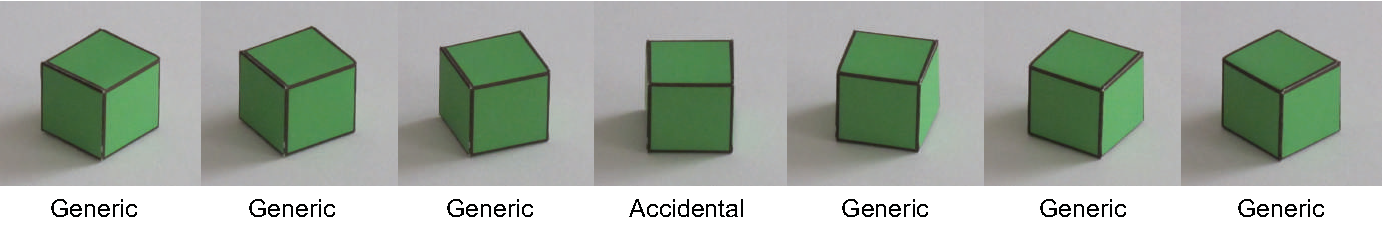
\includegraphics[width=1\linewidth]{figures/simplesystem/accidentalAlignments.pdf}
} 
\caption{The generic-view assumption breaks down for the central image, where the cube is precisely aligned with the camera axis.  
} 
\label{fig:accidentalAlignments}
\end{figure}


In \fig{\ref{fig:gradient}} we show the edges classified as vertical or horizontal using the edge angle. Anything that deviates from 2D verticality by more than 15 degrees is labeled as 3D horizontal.


We can now translate the inferred 3D edge orientation into linear constraints  on the global 3D structure. We will formulate these constraints in terms of $Y(x,y)$. Once $Y(x,y)$ is recovered we can also recover $Z(x,y)$ from \eqn{\ref{eq:projection}}. 

In a 3D vertical edge, using the projection equations, the derivative of $Y$ along the edge will be
\begin{eqnarray}
\partial Y / \partial y & = & 1/ \cos(\theta)
\label{eqn:derivative_Y_along_edge}
\end{eqnarray}


In a 3D horizontal edge, the coordinate $Y$ will not change. Therefore, the derivative along the edge should be zero:
\begin{eqnarray}
\partial Y / \partial {\bf t} & = & 0 
\label{eqn:derivative_Y_along_edge_hor}
\end{eqnarray}
where the vector $\bf t$ denotes direction tangent to the edge, ${\bf t}=(-n_y, n_x)$. 
\marginnote{\centerline{
\includegraphics[width=.4\linewidth]{figures/simplesystem/tangent.eps}
}}
We can write this derivative as a function of derivatives along the $x$ and $y$ image coordinates:
\begin{eqnarray}
\partial Y / \partial {\bf t} =  \nabla Y \cdot {\bf t} = -n_y \partial Y / \partial x + n_x \partial Y / \partial y
\label{eqn:derivative_Y_along_edge_tan}
\end{eqnarray}

When the edges coincide with occlusion edges, special care should be taken so that these constraints are only applied to the surface that owns the boundary. 

In this chapter, we represent the world coordinates $X(x,y)$, $Y(x,y)$, and $Z(x,y)$ as images where the coordinates $x,y$ correspond to pixel locations. Therefore, it is useful to approximate the partial derivatives in the same way that we approximated the image partial derivatives in equations (\ref{eq:image_partial_derivatives_aprox}). Using this approximation, \eqn{\ref{eqn:derivative_Y_along_edge}} can be written as follows:
\begin{eqnarray}
Y(x,y)-Y(x,y-1) & = & 1/ \cos(\theta)
\end{eqnarray}

Similar relationships can be obtained from equations (\ref{eqn:derivative_Y_along_edge_hor}) and (\ref{eqn:derivative_Y_along_edge_tan}).

\subsection{Constraint Propagation}
\label{sect:constraint}

Most of the image consists of flat regions where we do not have such edge constraints and we thus don't have enough local information to infer the surface orientation. Therefore, we need some criteria in order to propagate information from the  boundaries, where we do have information about the 3D structure, into the interior of flat image regions. This problem is common in many visual domains. 

\marginnote{
As shown on the left image bellow, an image patch without context is not enough to infer its 3D shape. 
The same patch shown in the original image (right):\\[6pt]
\centerline{
\includegraphics[width=.3\linewidth]{figures/simplesystem/cube_propagartion_1.eps}~~~~~~~~
\includegraphics[width=.3\linewidth]{figures/simplesystem/cube_propagartion_2.eps}
}
\\[6pt]
Information about its 3D orientation its propagated from the surrounding edges. 
}


In this case we will assume that the object faces are planar. Thus, flat image regions impose the following constraints on the local 3D structure:
\begin{eqnarray}
\partial^2 Y / \partial x^2 & = & 0  \\
\partial^2 Y / \partial y^2 & = & 0 \\  
\partial^2 Y / \partial y \partial x & = & 0 
\end{eqnarray}
That is, the second order derivative of $Y$ should be zero. As before, we want to approximate the continuous partial derivatives. The approximation to the  second derivative can be obtained by applying twice the first order derivative approximated by equations (\ref{eq:image_partial_derivatives_aprox}). The result is
$\partial^2 Y / \partial x^2 \simeq 2Y(x,y)-Y(x+1,y)-Y(x-1,y)$, and similarly for $\partial^2 X / \partial x^2$.

%$
%\left [
%\begin{matrix}
%-1 & 2 & -1 \\
%\end{matrix}
%\right ]
%$, which corresponds to 

\subsection{A Simple Inference Scheme}

All the different constraints described previously can be written as an overdetermined system of linear equations. Each equation will have the form:
\begin{eqnarray}
\mathbf{a}_i \mathbf{Y} = b_i
\end{eqnarray}
where $\mathbf{Y}$ is a vectorized version of the image $Y$ (i.e., all rows of pixels have been concatenated into a flat vector). Note that there might be many more equations than there are image pixels.

We can translate all the constraints described in the previous sections into this form. For instance, if the index $i$ corresponds to one of the pixels inside one of the planar faces of a foreground object, then there will be three equations. One of the planarity constraint can be written as $\mathbf{a}_i = [0, \dots, 0, -1, 2, -1, 0, \dots, 0]$, $b_i=0$, and analogous equations can be written for the other two.

We can solve the system of equations by minimizing the following cost function:
\begin{eqnarray}
J = \sum_i (\mathbf{a}_i\mathbf{Y} - b_i)^2
\end{eqnarray}
where the sum is over all the constraints. 

If some constraints are more important than others, it is possible to also add a weight $w_i$.
\begin{eqnarray}
J = \sum_i w_i (\mathbf{a}_i \mathbf{Y} - b_i)^2
\end{eqnarray}

Our formulation has resulted on a big system of linear constraints (there are more equations than there are pixels in the image). It is convenient to write the system of equations in matrix form:
\begin{eqnarray}
\mathbf{A} \mathbf{Y}  = \mathbf{b}
\end{eqnarray}
where row $i$ of the matrix ${\bf A}$ contains the constraint coefficients $\mathbf{a}_i$. The system of equations is overdetermined ($\mathbf{A}$ has more rows than columns). We can use the pseudoinverse to compute the solution:
\begin{eqnarray}
\bf Y = (\mathbf{A}^T \mathbf{A})^{-1} \mathbf{A}^T \mathbf{b}
\end{eqnarray}
This problem can be solved efficiently as the matrix $\mathbf{A}$ is very sparse (most of the elements are zero).

\subsection{Results}

\Fig{\ref{fig:worldCoordinates}} shows the resulting world coordinates $X(x,y)$, $Y(x,y)$, $Z(x,y)$ for each pixel. The world coordinates are shown here as images with the gray level coding the value of each coordinate (black corresponds to the value 0). 

\begin{figure}[t]
\centerline{
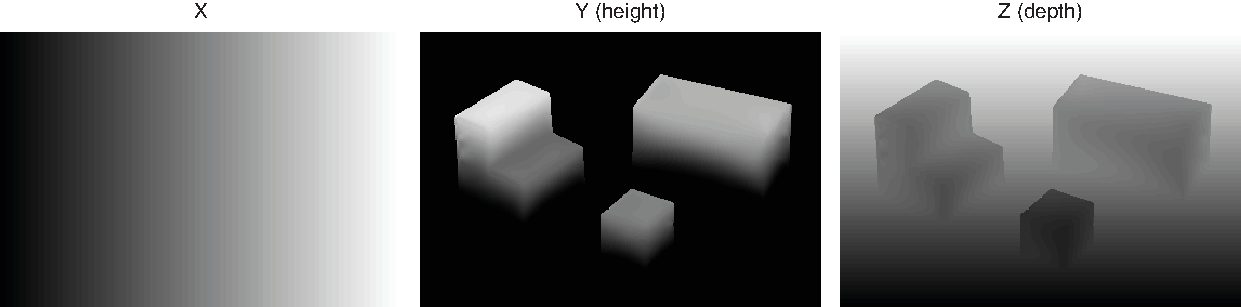
\includegraphics[width=1\linewidth]{figures/simplesystem/worldCoordinates.pdf}
} 
\caption{The solution to our vision problem for the input image of \fig{\ref{fig:edgeLabeling}}.
%the assumptions and inference scheme described below leads to these estimates of 3D world coordinates at each image location. 
World coordinates $X$, $Y$, and $Z$ are shown as images.} 
\label{fig:worldCoordinates}
\end{figure}

There are a few things to reflect on: 
\begin{itemize}
\item It works. At least it seems to work pretty well. Knowing how well it works will require having some way of evaluating performance. This will be important.
\item But it cannot possibly work all the time. We have made lots of assumptions that will work only in this simple world. The rest of the book will involve upgrading this approach to apply to more general input images.
\end{itemize}

Despite that this approach will not work on general images, many of the general ideas will carry over to more sophisticated solutions (e.g., gather and propagate local evidence).  One thing to think about is if information about 3D orientation is given in the edges, how does that information propagate to the flat areas of the image in order to produce the correct solution in those regions? 


Evaluation of performance is a very important topic. Here, one simple way to visually verify that the solution is correct is to render the objects under new view points. \Fig{\ref{fig:views}} shows the reconstructed 3D scene rendered under different view points to show that the 3D structure has been accurately captured. 

\begin{figure}[!h]
\centerline{
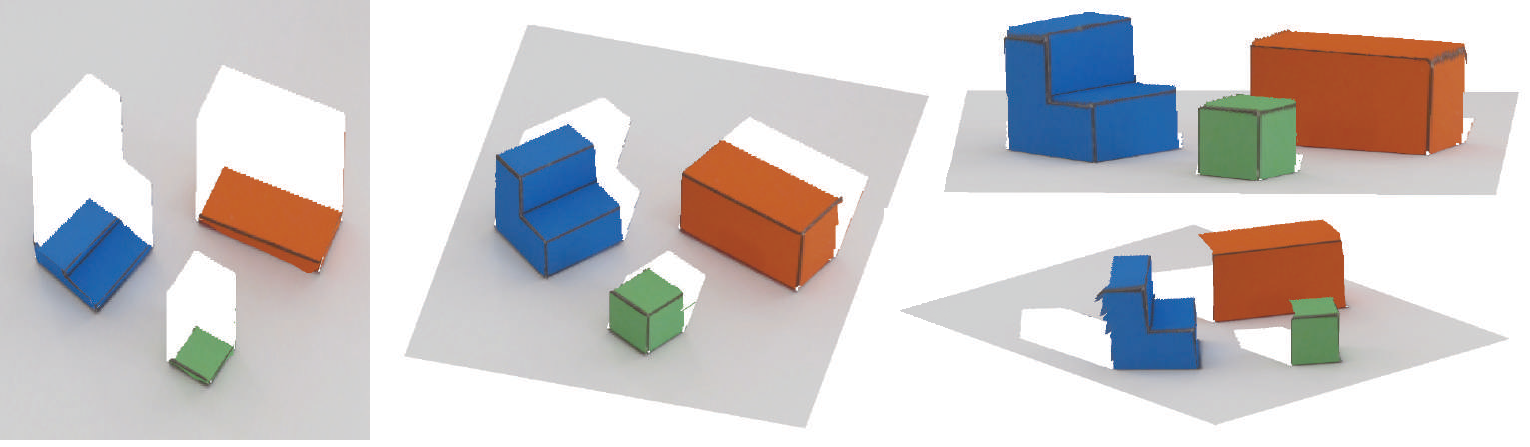
\includegraphics[width=1\linewidth]{figures/simplesystem/views.pdf}
} 
\caption{To show that the algorithm for 3D interpretation gives reasonable results we can re-render the inferred 3D structure from different viewpoints.} 
\label{fig:views}
\end{figure}

\section{Generalization}

One desired property of any vision system is it ability to {\bf generalize} outside of the domain for which it was designed to operate. In the approach presented in this chapter, the domain of images the algorithm is expected to work is defined by the assumptions described in \sect{\ref{sec:algo_simple_world}}. Later in the book, when we describe learning-based approaches, the training dataset will specify the domain. 
\marginnote{{\bf Out of domain generalization} refers to the ability of a system to operate outside the {\bf domain} for which it was designed.}
What happens when assumptions are violated? Or when the images contain configurations that we did not consider while designing the algorithm?



Let's run the algorithm with shapes that do not satisfy the assumptions that we have made for the simple world. \Fig{\ref{fig:out_of_domain}} shows the result when the input image violates several assumptions we made (shadows are not soft and the green cube occludes the red one) and when it has one object on top of the other, a configuration that we did not consider while designing the algorithm. In this case the result happens to be good, but it could have gone wrong.



\begin{figure}[t]
\centerline{
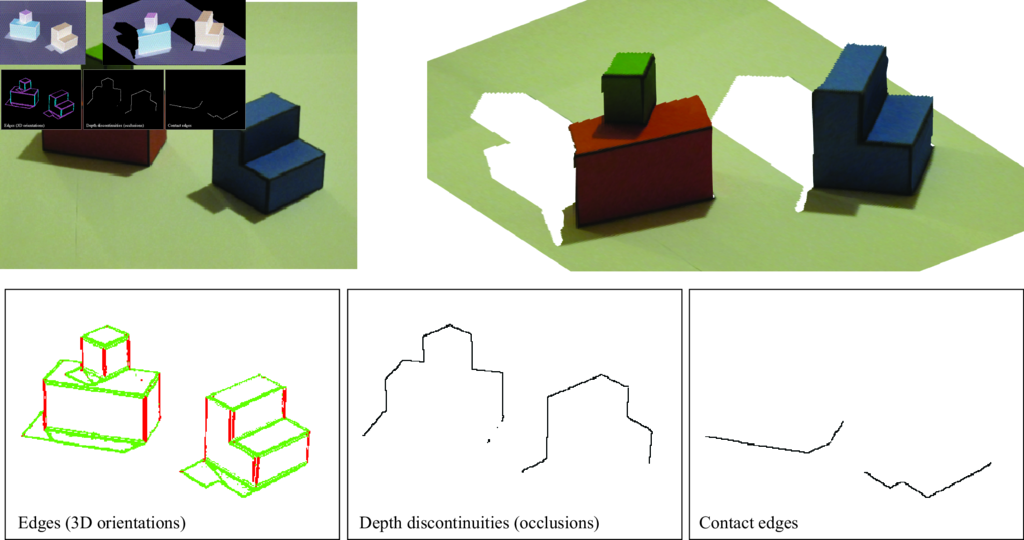
\includegraphics[width=1\linewidth]{figures/simplesystem/out_of_domain_example.eps}
} 
\caption{Reconstruction of an out-of-domain example. The input image violates several assumptions we made (shadows are not soft and the green cube occludes the red one) and it has one object on top of the other, a configuration that we did not consider while designing the algorithm. 
%In this case the result happens to be good, but it could have gone wrong easily.
} 
\label{fig:out_of_domain}
\end{figure}

\Fig{\ref{fig:impossible}} shows the {\em impossible steps} inspired from \cite{Adelson99}. On the left side, this shape looks rectangular and the stripes appear to be painted on the surface. On the right side, the shape looks as though it has steps, with the stripes corresponding to shading due to the surface orientation. In the middle, the shape is ambiguous. 
\Fig{\ref{fig:impossible}} shows the reconstructed 3D scene for this unlikely image. The system has tried to approximate the constraints, but for this shape it is not possible to exactly satisfy all the constraints.  


\begin{figure}[t]
\centerline{
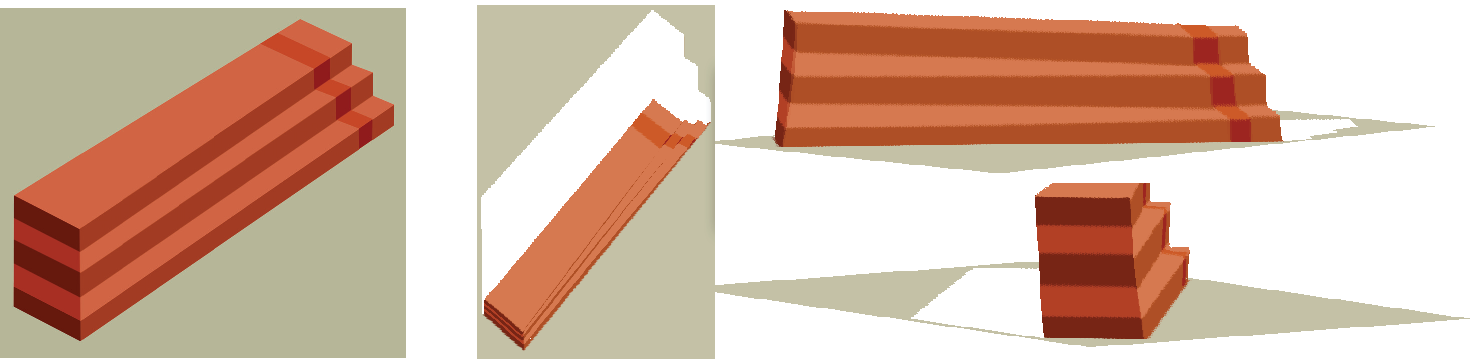
\includegraphics[width=1\linewidth]{figures/simplesystem/steps.pdf}
} 
\caption{Reconstruction of an impossible figure (inspired from \cite{Adelson99}): the reconstruction agrees with our 3D perception.} 
\label{fig:impossible}
\end{figure}


\section{Concluding Remarks}

Despite having a 3D representation of the structure of the scene, the system is still unaware of the fact that the scene is composed of a set of distinct objects. For instance, as the system lacks a representation of which objects are actually present in the scene, we cannot visualize the occluded parts. The system cannot do simple tasks like counting the number of cubes. 

A different approach to the one discussed here is model-based scene interpretation, where we could have a set of predefined models of the objects that can be present in the scene and the system can try to decide if they are present or not in the image, and recover their parameters (i.e., pose, color).

Recognition allows indexing properties that are not directly available in the image. For instance, we can infer the shape of the invisible surfaces. Recognizing each geometric figure also implies extracting the parameters of each figure (i.e., pose, size).

%[NOTE: This section needs to be developed a bit more. Or perhaps removed from here?]

%% FIGURE: see what happens with real images. See that the simple vision problem is not that simple.

%\section{Conclusion}


%\Appendix{Linear filtering}

%Convolution

%Writing a filter in matrix form


%\section{From objects back to the image}

Given a detailed representation of the world, we could render the image back, or at least some aspects of it. We can check that we are understanding things correctly and judge if we can make verifiable predictions, such as what we would see if we looked behind the object. Closing the loop between interpretation and input will be productive at some point.

In this chapter, besides introducing some useful vision concepts, we also made use of mathematical tools from algebra and calculus that you should be familiar with.

%\newcommand{\hwproblem}[2] {\noindent \\ {\bf #1} {\it #2}}

\newcommand{\textbox}[1]{\hfill\rule{0ex}{0.01ex}
 \centerline{\fbox{\parbox{\textwidth}{#1}}}}

\clearpage
{\Large Exercises}

% Administration
\textbox{
We provide a python notebook with the code to be completed. You can
run it locally or in Colab. To use Colab, upload it to Google Drive
and select `open in colab',  which will allow you to complete the
problems without setting up your own environment. Once you have
finished, copy the code sections that  you have completed\ as
screenshots to the report. \\
}
\vspace{0.2cm}


\hwproblem{Problem 1}{Perspective and orthographic projections}

The goal of this first exercise is to take images with different settings of a camera to create pictures with perspective projection and with orthographic projection. Both pictures should cover the same piece of the scene. You can take pictures of real places or objects (e.g. your furniture).% (e.g., the street, a living room, ...) or you can also create your own simple world (e.g., you can print \texttt{simpleWorld.pdf} and create your own scenes. I recommend printing on matte paper).

To create pictures with orthographic projection you can do two things: 1) use the zoom of the camera, 2) crop the central part of a picture. You will have to play with the distance between the camera and the scene, and with the zoom or cropping so that both images look as similar as possible, only differing in the type of projection (similar to figure 2.2).

Submit the two pictures and clearly label parts of the images that reveal their projection types.


\hwproblem{Problem 2}{Orthographic projection equations} 

Recall the parallel projection equations:
\begin{gather}
    x = \alpha  X + x_0\\
    y = \alpha (\cos(\theta)Y - \sin(\theta)Z) +y_{0}
\end{gather}
which relate the coordinates of a point in the 3D world to the image coordinates of an orthogonal camera rotated by $\theta$ over the $X$-axis.

Show that the  equations emerge naturally from a series of transformations
applied to the 3D world coordinates $(X,Y,Z)$, of the form:
\begin{gather}
\left[
  \begin{array}{c}
    x \\
    y
  \end{array}
\right] = \alpha \cdot P \cdot R_x(\theta) \cdot
\left[
  \begin{array}{ccc}
    X \\
    Y \\
    Z
  \end{array}
\right] +
\left[
  \begin{array}{c}
    x_0 \\
    y_0
  \end{array}
\right]
\end{gather}
Where $R_x(\theta)$ is a $3\times 3$ matrix corresponding to a rotation over the $X$ axis, $P$ is a $2 \times 3$ matrix corresponding to the orthogonal projection and $\alpha$ is  a scaling factor to account for the size
of the
camera sensor, which is a single scalar when the pixels are square (assumed in this case).  

Then, find $\alpha$, $x_0$ and $y_0$ when the world point $(0, 0, 0)$ projects onto  $(0, 0)$ \ (which corresponds to the center of the image) and the point $(1, 0, 0)$ projects onto $(3, 0)$.



\hwproblem{Problem 3}{Edge and surface constraints}

In Sect.~\ref{sect:constraint}, we have written down the constraints for $Y(x, y)$. Briefly derive the constraints for $Z(x, y)$ along vertical edges, horizontal edges, and flat surfaces.


\hwproblem{Problem 4}{Complete the code}

Fill in the missing lines in the notebook: \texttt{Ch2.ipynb}, and include them in the report as screenshots. First, find a way to classify edges as vertical or horizontal edges. Next, fill in the rest of the conditions of the constraint matrix. The constraints for when the pixel is on the ground have already been done for you as an example. Put the kernel in \texttt{Aij} and the value you expect in \texttt{b} (the conversion to a linear system is done for you later so you don't need to worry about that part).

You only need to modify the locations marked with a \texttt{TODO} comment.

Please make sure to also include your answers for \texttt{vertical\_edges}, \texttt{horizontal\_edges}, and your formulations for \texttt{Aij} and \texttt{b} for the different constraints in the report.

\hwproblem{Problem 5}{Run the code} 

Select some of the images included with the code and show some new viewpoints for them.

Optional: You can also try with new images taken by you if you decide to create your own simple world.

\hwproblem{Problem 6}{Violating simple world assumptions} (1 point)

Find one example from the four images provided with the problem set (\texttt{img1.jpg}, ..., \texttt{img4.jpg}) when the recovery of 3D information fails. Include the image and the reconstruction in your writeup, and explain why it fails.

\hwproblem{Research problem} {The real world} [optional]

\textit{A research problem is a question for which we do not know the answer. In fact, there might not
even be an answer. This question is optional and could be extended into a larger course project.}

The goal of this problem is to test the 3D reconstruction code with real images. A number of the assumptions we have made will not work when the input is real images of a more complex scene. For instance, the simple strategy of differentiating between foreground and background segmentation will not work with other scenes.

Try taking pictures of real-world scenes and propose modifications to the scheme proposed in this lecture so that you can get some better 3D reconstructions. The goal is not to build a general system, but to be able to handle a few more situations.

 
